Každý model se skládá ze tří základních složek a to vertices, edges a faces, které definují celkový tvar a vzhled. Pro tvorbu modelů do hry Codeventure je využit Low Poly styl, protože se jedná o modely s menším počtem polygonů a díky tomu jsou vymodelované objekty více optimalizované. Pro tvorbu objektů byl využit software Blender, který je ideální volbou pro tvorbu 3D grafických podkladů pro hru. Herní modely jsou využity v Unity a mobilní aplikaci.

\subsection{Box modeling}
Box modeling je technika modelování, při které se využívají pouze základní objekty (jako je krychle, koule, atd.). Tento objekt se poté používá k dosažení finálního tvaru objektu dle připraveného návrhu. Celkový cyklus se opakuje s každým novým prvkem a jednotlové modely se poté kombinují k dosažení cílového tvaru.

\subsection{Low poly}
Pro tvorbu jednotlivých herních modelů využíváme styl Low poly, který nám nabízí vysokou optimalizaci pro herní využití. Low poly modely vypadají jednoduché, přičemž představují zákaldní tvar představované věci.

\subsection{Jednotlové herní modely}
Na začátku tvoření modelů bylo hlavní vybrat dobu, či místo, do které hru zasadíme. Drželi jsme se proto námi vytvořeného příběhu o magickém světe a kouzelníkovi zachraňujícím svoji planetu.

\subsubsection{Postavy}
\subsubsubsection{Hlavní postava}
Model hlavní postavy byl klíčovy, protože představuje hráče a jeho postup hrou doprovází na každém kroku. Jak můžeme vidět na obr. \ref{fig:hlavni-postava}, tak model kouzelníka je hravý a jednoduchý. K modelu je vytvořena také sada animací pro jednotlivé pohybové operace ve hře.

\begin{figure}[h]
    \centering
    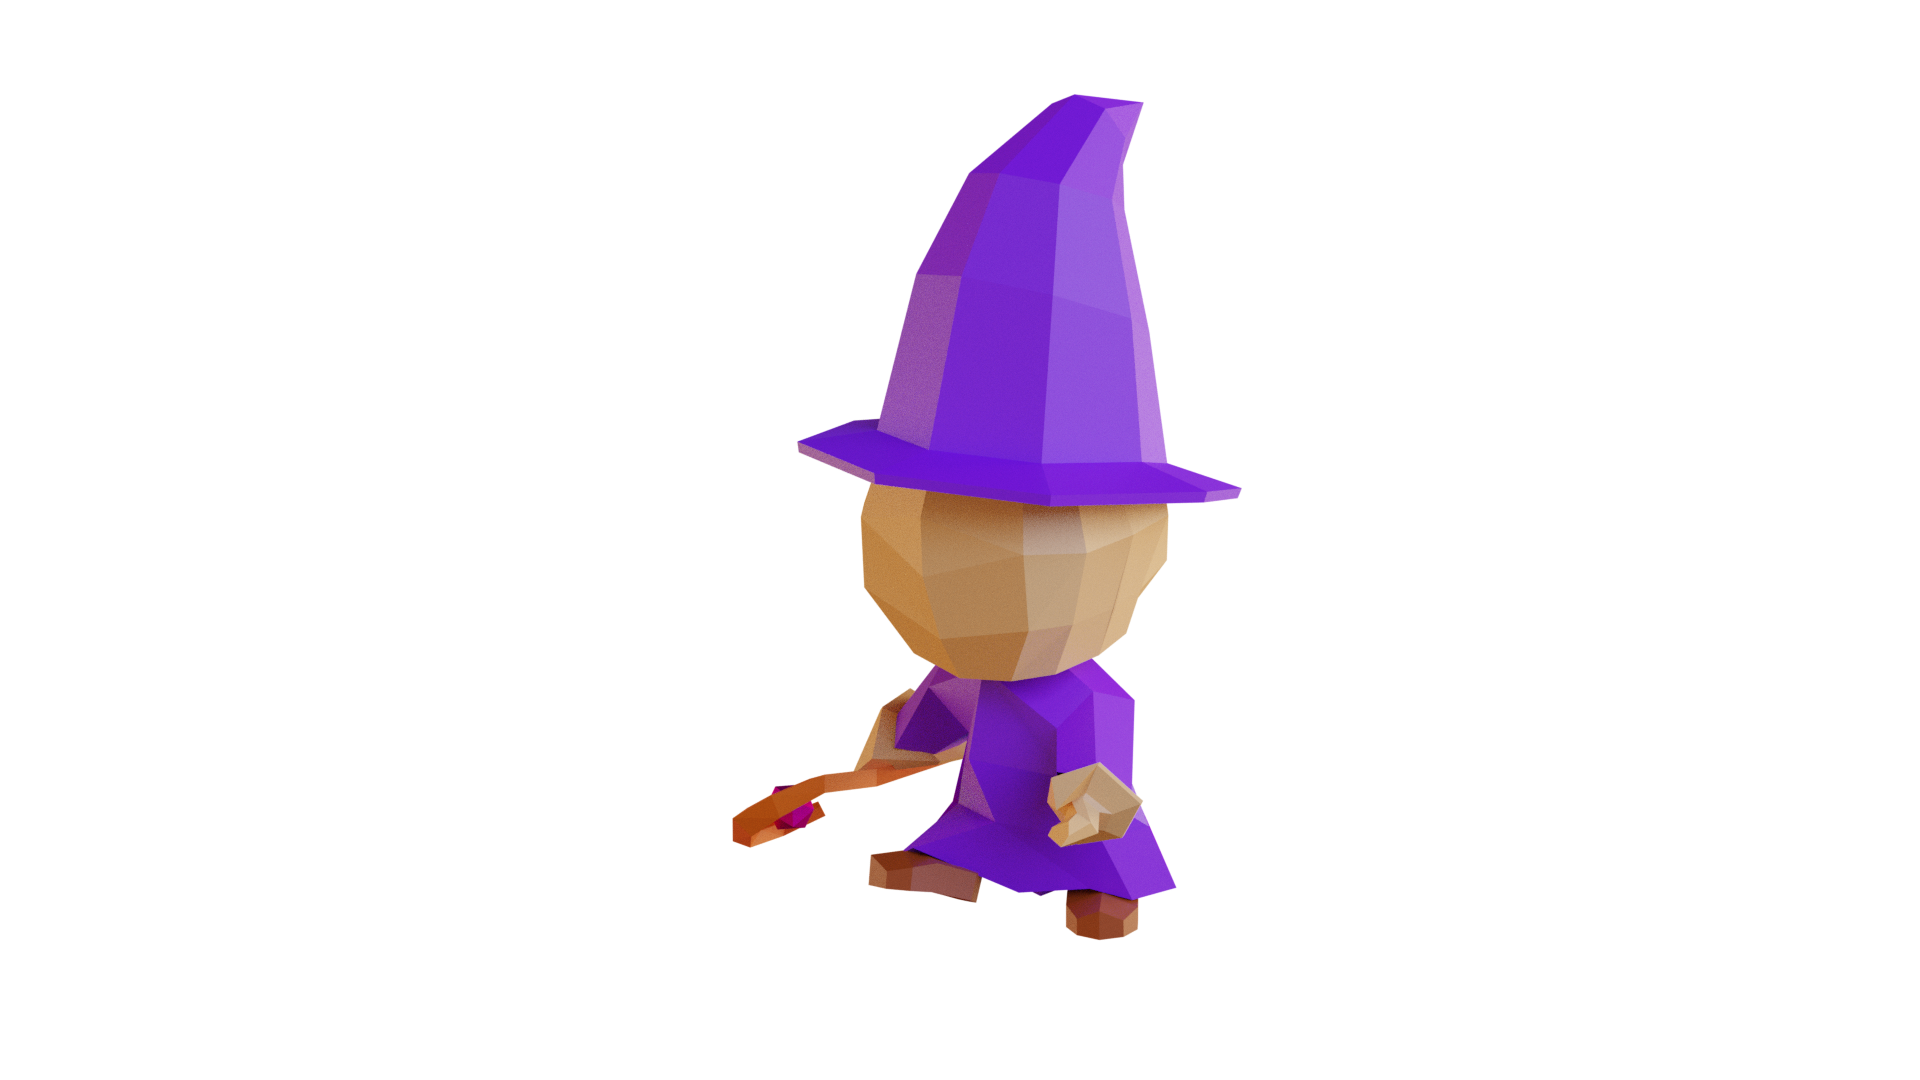
\includegraphics[width=0.6\textwidth]{img/hlavni-postava.png}
    \caption{Model hlavní postavy.}
    \label{fig:hlavni-postava}
\end{figure}

\subsubsubsection{Nepřátelé}
Každý ostrov má sadu nepřátel, které hráč může nalézt v jednotlivých úrovních. Nepřátelé mají za úkol hráči ztížit průchod úrovní. Jednotlivé nepřátelské jednotky mají sadu animací. Modely nepřátel můžeme vidět na obr. \ref{fig:nepritel-golem}, nebo obr. \ref{fig:nepritel-cerv}.

\begin{figure}[h]
    \centering
    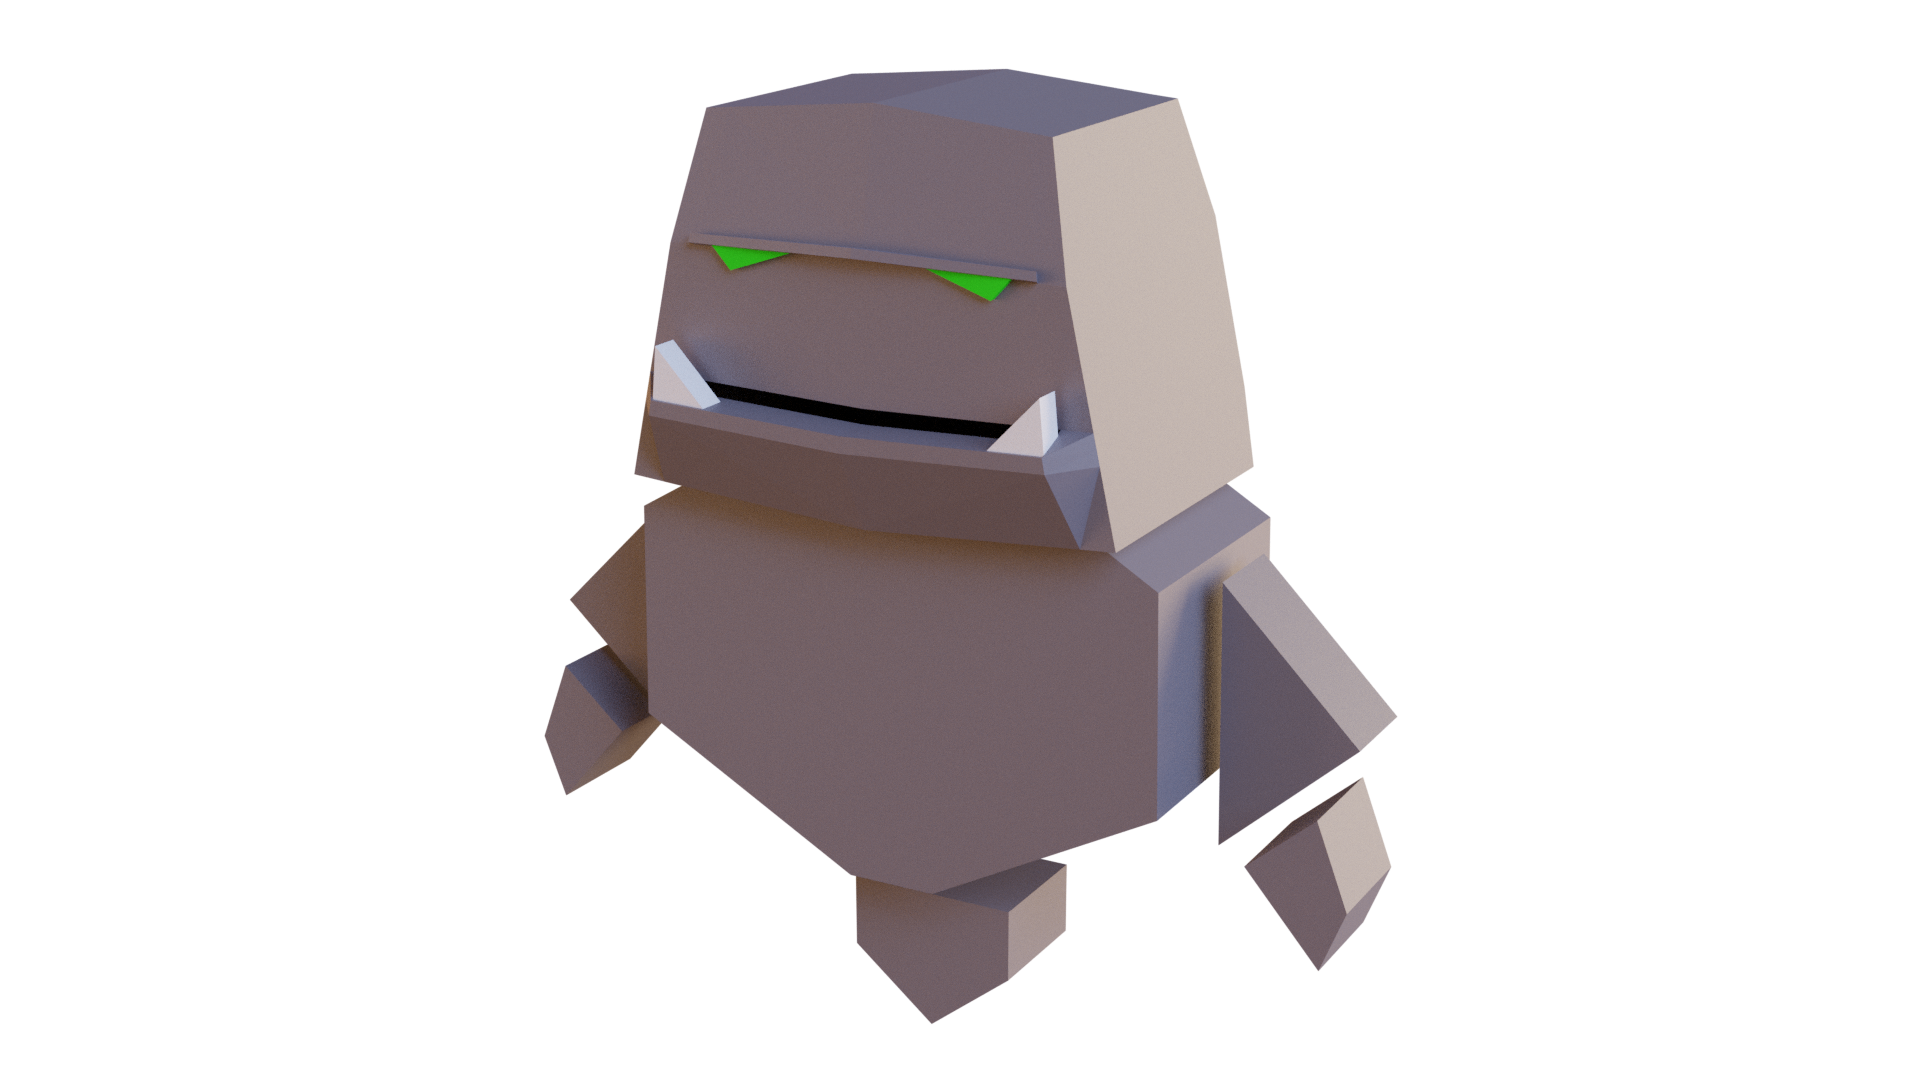
\includegraphics[width=0.6\textwidth]{img/nepritel-golem.png}
    \caption{Model nepřítele - Golem.}
    \label{fig:nepritel-golem}
\end{figure}

\begin{figure}[h]
    \centering
    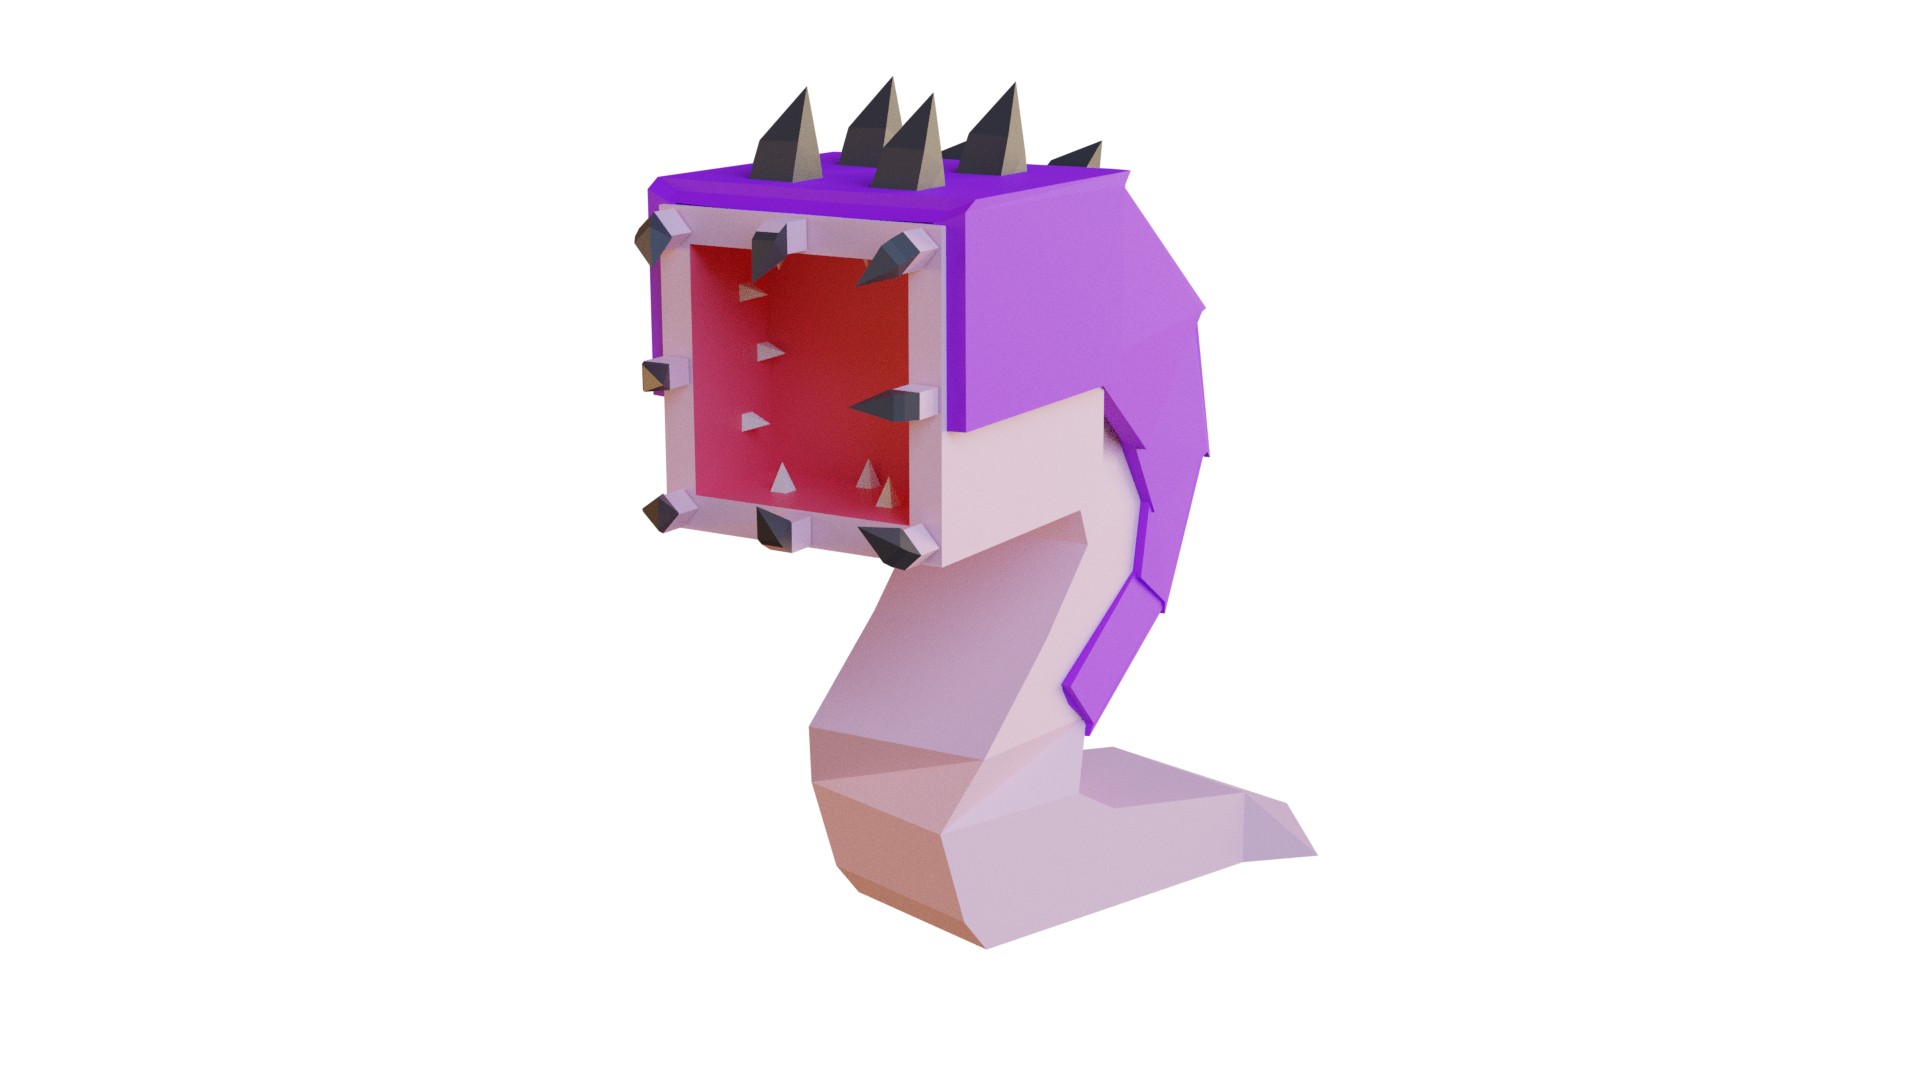
\includegraphics[width=0.6\textwidth]{img/nepritel-cerv.png}
    \caption{Model nepřítele - Červ.}
    \label{fig:nepritel-cerv}
\end{figure}

\subsubsection{Ostrovy}
Jednotlivé modely ostrovů představují přírodní elementy. Dle jednotlivých elementů jsou zbarvené a doplněné o modely, které můžeme ve spojitosti s tímto elementem nalézt. Modely ostrovů jsou využité v mobilni aplikaci, jako je vidět na obr. \ref{fig:mobilni-aplikace-ostrov} Dominantou každého ostrova je krystal, který musí hráč získat pro úspěšné splnění. Ukázka zmiňovaných modelů obr. \ref{fig:nature-island}, obr. \ref{fig:fire-island} a obr. \ref{fig:winter-island}.

\begin{figure}[h]
    \centering
    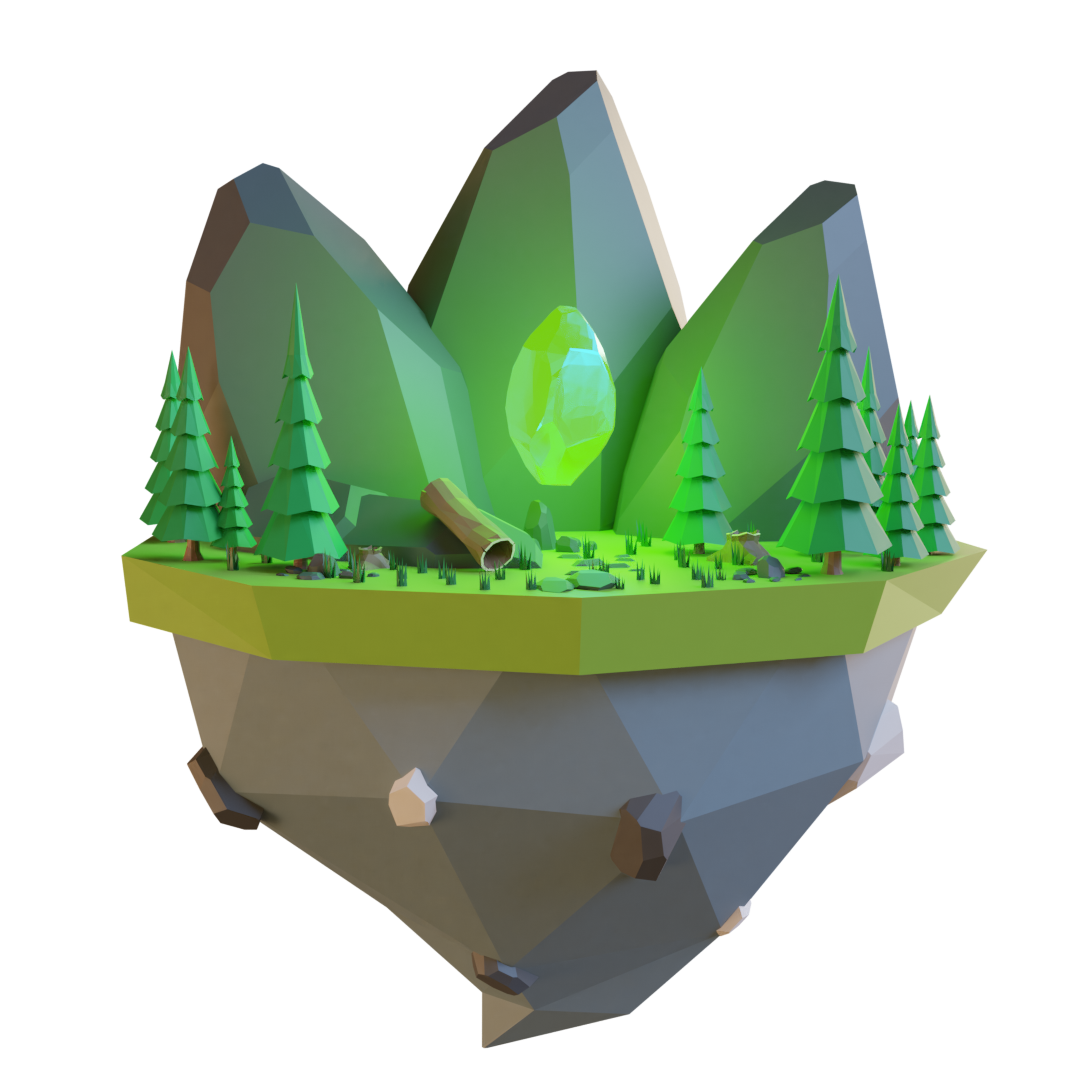
\includegraphics[width=0.6\textwidth]{img/NatureIsland.png}
    \caption{Model ostrova - Zemní ostrov.}
    \label{fig:nature-island}
\end{figure}

\begin{figure}[h]
    \centering
    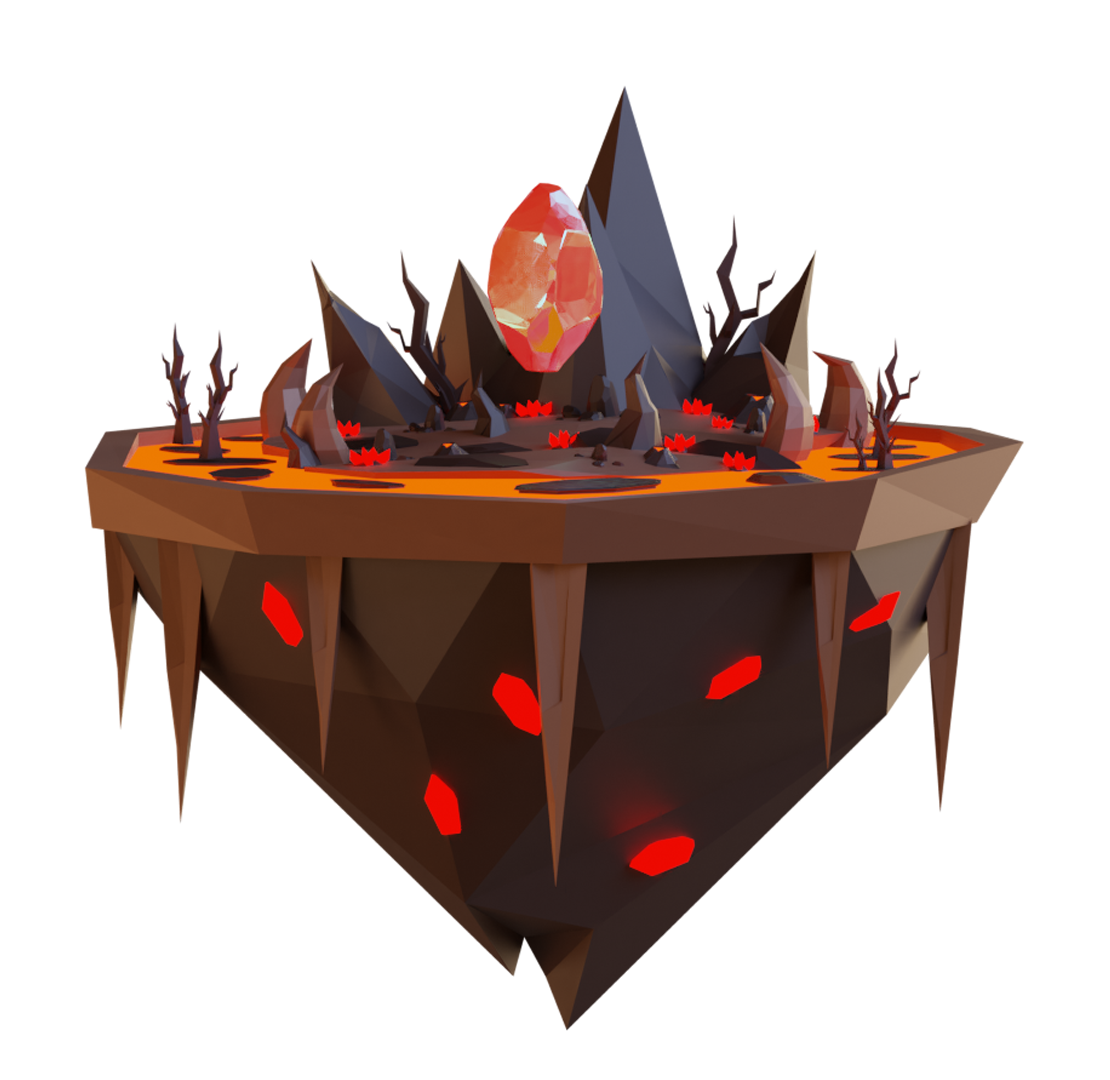
\includegraphics[width=0.6\textwidth]{img/FireIsland.png}
    \caption{Model ostrova - Ohnivý ostrov.}
    \label{fig:fire-island}
\end{figure}

\begin{figure}[h]
    \centering
    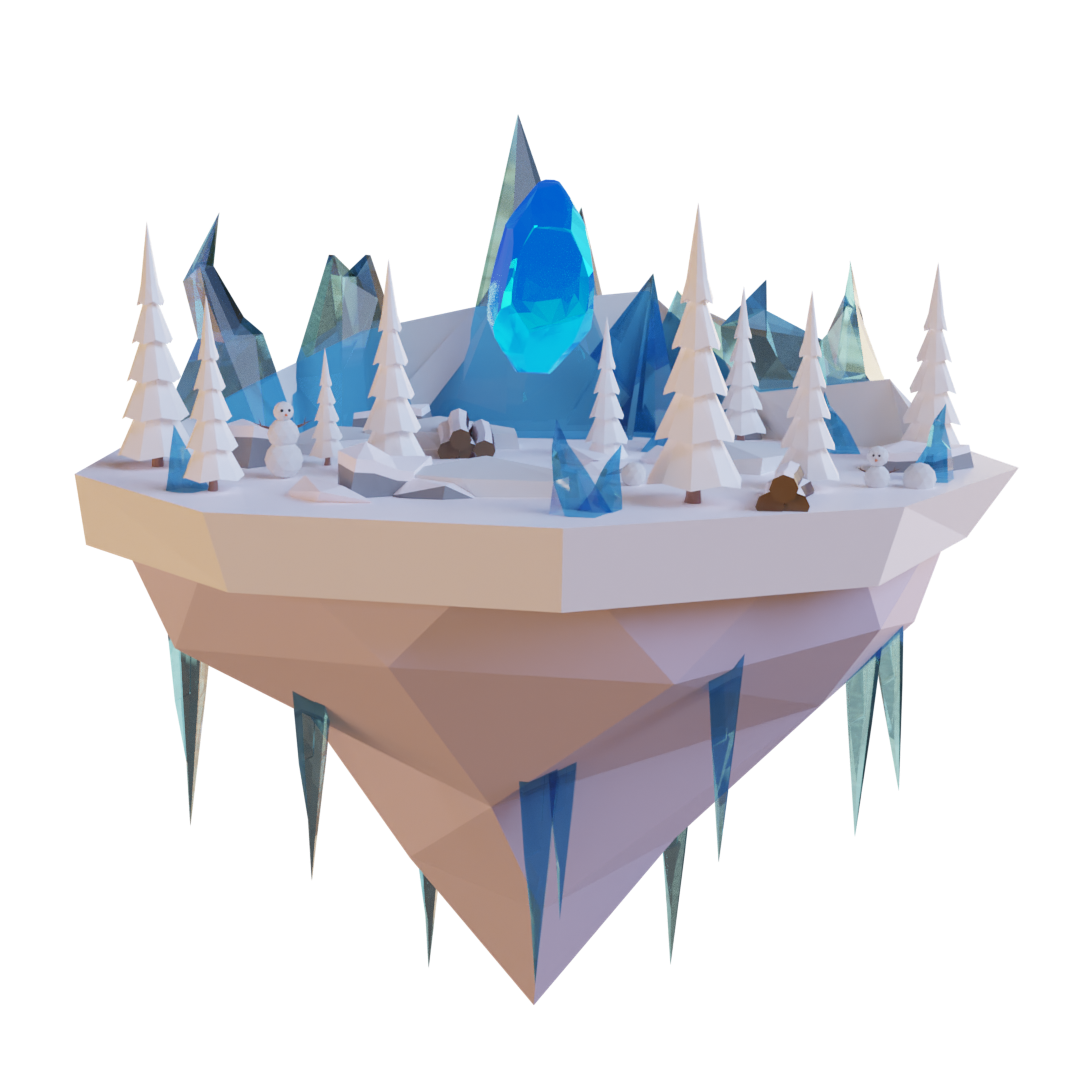
\includegraphics[width=0.6\textwidth]{img/WinterIsland.png}
    \caption{Model ostrova - Zimní ostrov.}
    \label{fig:winter-island}
\end{figure}

\begin{figure}[h]
    \centering
    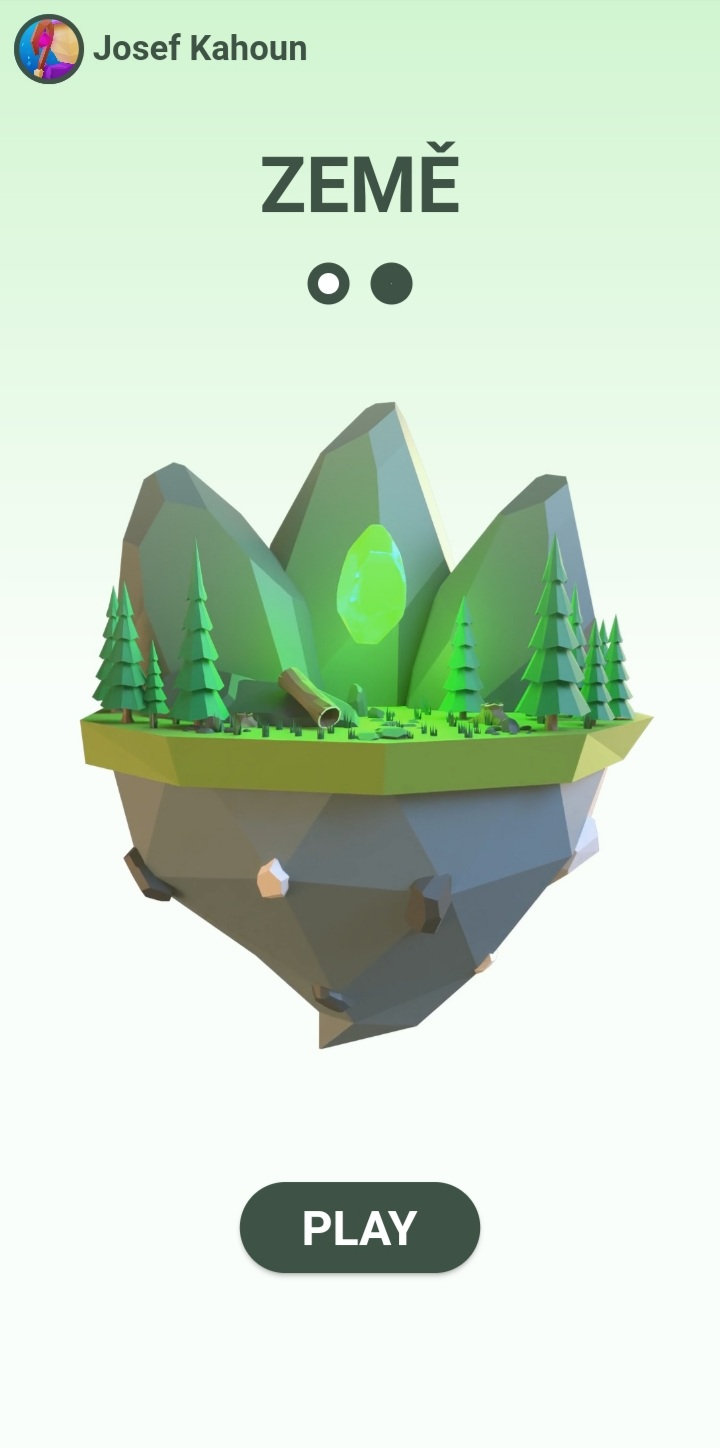
\includegraphics[width=0.6\textwidth]{img/mobilni-aplikace-ostrov.jpg}
    \caption{Model ostrova v mobilní aplikace.}
    \label{fig:mobilni-aplikace-ostrov}
\end{figure}

\subsubsubsection{Úrovně}
Jednotlivé úrovně tvoří mřížku, jako je vidět na obr. \ref{fig:model-levelu}. Úrovně představují stejný element, jako je ostrov, ke kterému patří. Na herních plošinách se odehrává celá hra, kde hráč skládá sekvence kódů. Jednotlivé pole úrovně slouží jako umistitel herních postav, bariér, cest, či ukazatel cíle. Prostředí okolo herních plošinek je doplněno o modely mateřského ostrova. Úkázka herního prostředí jednotlivé úrovně, které můžete vidět na obr. \ref{fig:model-levelu}

\begin{figure}[h]
    \centering
    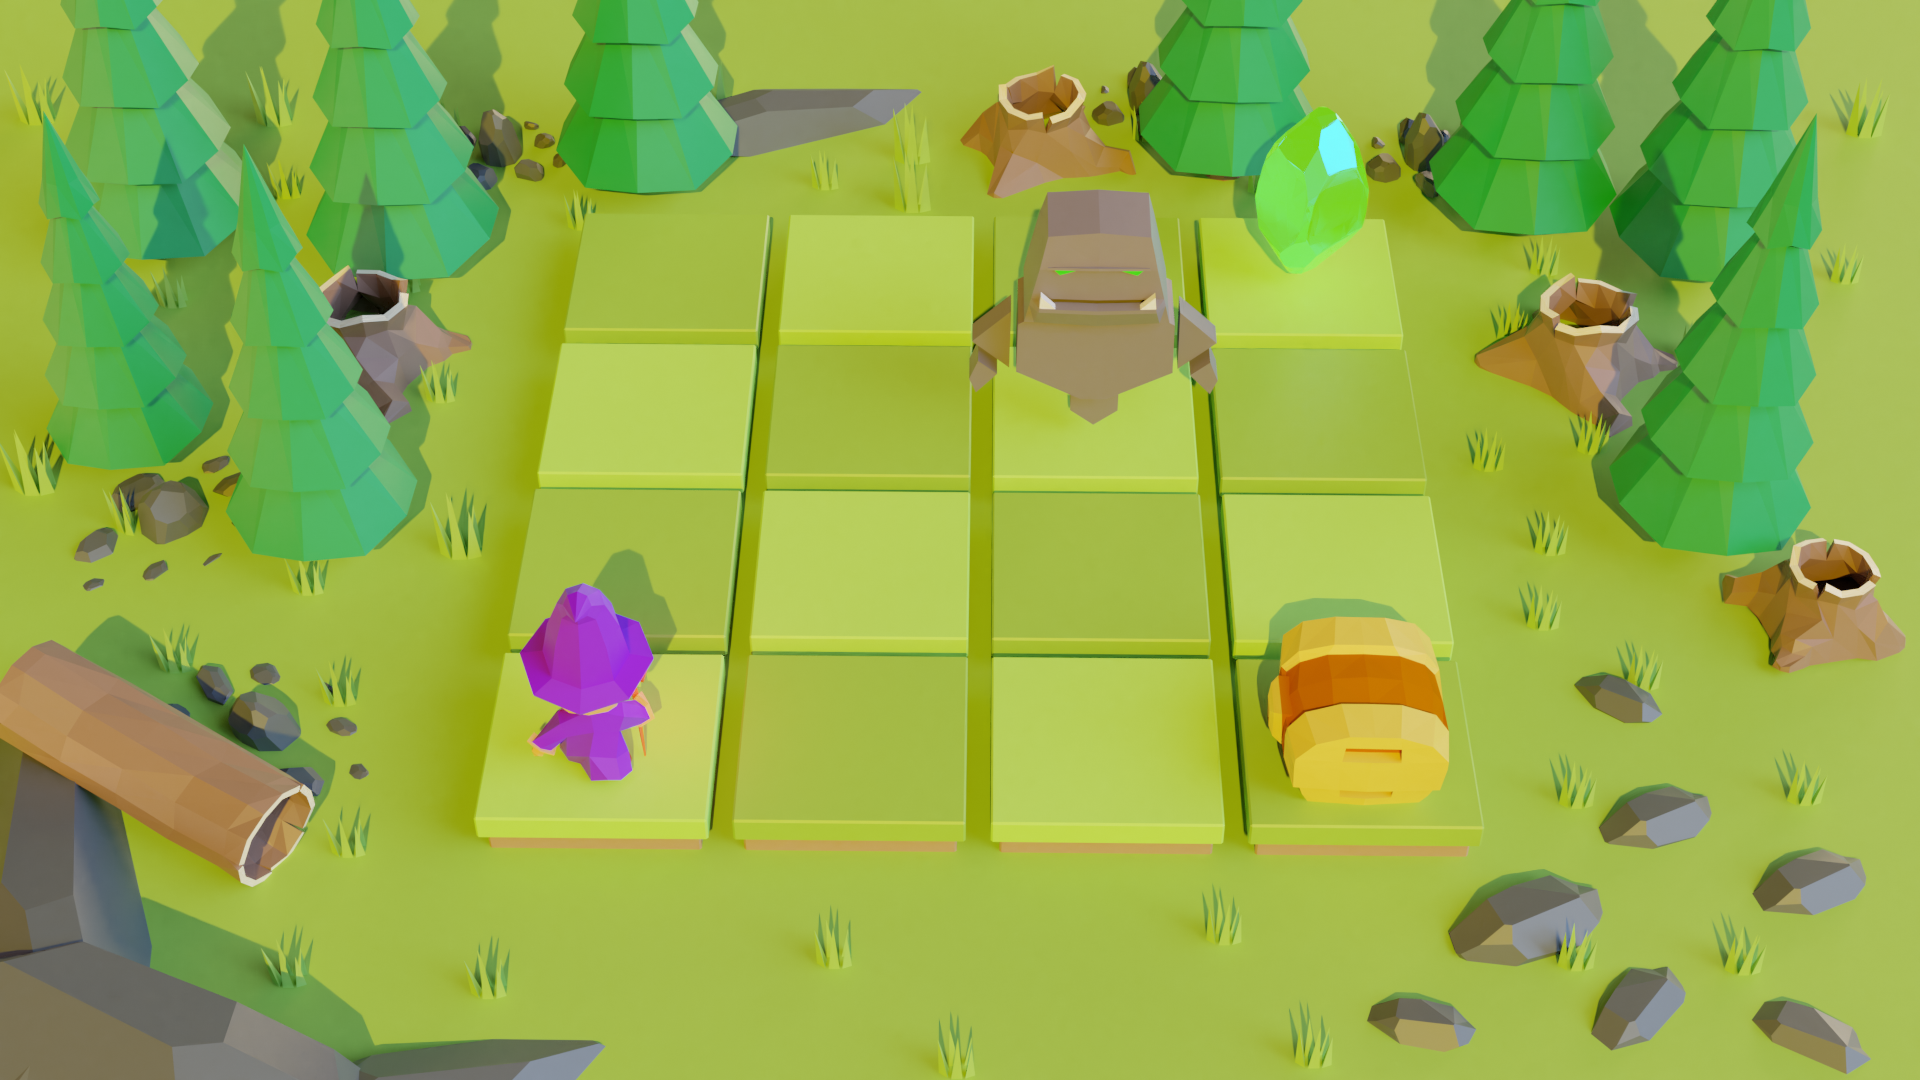
\includegraphics[width=0.6\textwidth]{img/model-levelu.png}
    \caption{Model úrovně.}
    \label{fig:model-levelu}
\end{figure}